\section{Максимальный поток}
\subsection{Условие задания}
Решить задачу на нахождение максимального потока любым алгоритмом.
Подготовить примеры, демонстрирующие работу алгоритма в разных случаях.

\subsection{Примеры исходного кода}
Для выполнения задания был реализован метод
\mitext{taskEleven()}, а также вспомогательный метод
\mitext{findAugmentingPath()}. С целью экономии места,
код \mitext{findAugmentingPath()} расположен в приложении
\ref{app:max-flow}.
\begin{minted}{typescript}
/**
 * Метод, находящий максимальный поток а графе, используя алгоритм
 * Форда-Фалкерсона.
 * @param source источник
 * @param sink сток
 */
taskEleven(source: string, sink: string): number {
  if (!this.exists(source)) {
    throw new NodeNotExists(source)
  }
  if (!this.exists(sink)) {
    throw new NodeNotExists(sink)
  }

  // создать остаточный граф с теми же вершинами, что и в изначальном
  const resGraph: Map<string, Map<string, number>> = new Map()
  for (const [vertex, edges] of this.adj.entries()) {
    resGraph.set(vertex, new Map(edges))
  }

  let maxFlow = 0

  // расширять поток, пока есть расширяющий путь
  let path = this.findAugmentingPath(resGraph, source, sink)
  while (path.length > 0) {
    // найти минимальную пропускную способность
    const minCapacity = this.findMinCapacity(resGraph, path)

    // обновить остаточный граф вычитанием минимальной пропускной способности
    for (let i = 0; i < path.length - 1; i++) {
      const u = path[i]
      const v = path[i + 1]

      resGraph.get(u)!.set(v, resGraph.get(u)!.get(v)! - minCapacity)

      // добавить обратную дугу с отрицательным весом
      if (!resGraph.has(v)) {
        resGraph.set(v, new Map())
      }

      if (!resGraph.get(v)!.has(u)) {
        resGraph.get(v)!.set(u, 0)
      }

      resGraph.get(v)!.set(u, resGraph.get(v)!.get(u)! + minCapacity)
    }

    // обновить значение максимального потока
    maxFlow += minCapacity

    // найти максимальный расширяющий путь
    path = this.findAugmentingPath(resGraph, source, sink)
  }

  return maxFlow
}
\end{minted}

\subsection{Краткое описание алгоритма}
Создается остаточный граф, который изначально совпадает с оригинальным графом,
но все веса обратных ребер устанавливаются в 0.

Алгоритм производит поиск расширяющих путей в остаточном графе с помощью вспомогательного
метода \mitext{findAugmentingPath()}. Этот метод использует обход в ширину (BFS) для нахождения
пути от источника к стоку, учитывая только те ребра, у которых остаточная пропускная способность больше нуля.

Если найден расширяющий путь, вычисляется минимальная пропускная способность на этом пути. Затем
обновляются значения остаточных пропускных способностей вдоль этого пути путем вычитания минимальной
пропускной способности.

Процесс поиска расширяющих путей и их обновления в остаточном графе повторяется до тех пор, пока не
удастся найти больше расширяющих путей. В процессе выполнения алгоритма суммируется пропускная
способность всех найденных путей, что и является максимальным потоком.

\subsection{Примеры входных и выходных данных}
\subsubsection{Входные данные}
Простой граф с двумя вершинами и одним направленным ребром.
\begin{figure}[H]
  \begin{minipage}{0.5\textwidth}
    \centering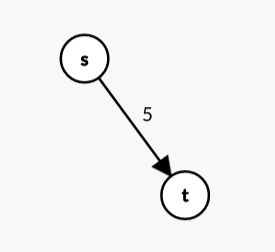
\includegraphics[width=0.6\linewidth]{figs/task-11/graph-ff-1.png}
  \end{minipage}
  \begin{minipage}{0.5\textwidth}
    \centering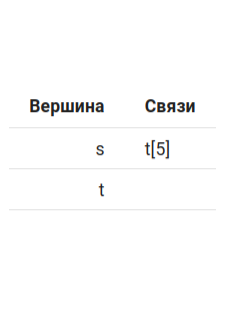
\includegraphics[width=0.6\linewidth]{figs/task-11/adj-ff-1.png}
  \end{minipage}
  \caption{Ориентированный взвешенный граф}
\end{figure}

\begin{minted}{js}
{
  "weighted": true,
  "oriented": true,
  "adj": {
    "s": {
      "t": 5
    },
    "t": {}
  }
}
\end{minted}

\subsubsection{Выходные данные}
\begin{figure}[H]
  \centering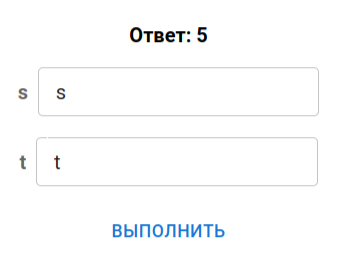
\includegraphics[width=0.3\textwidth]{figs/task-11/res-ff-1.png}
  \caption{Результат работы}
\end{figure}

\subsubsection{Входные данные}
Более сложный граф с четырьмя вершинами и несколькими ребрами.
\begin{figure}[H]
  \begin{minipage}{0.5\textwidth}
    \centering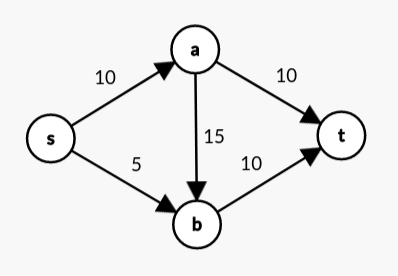
\includegraphics[width=0.8\linewidth]{figs/task-11/graph-ff-2.png}
  \end{minipage}
  \begin{minipage}{0.5\textwidth}
    \centering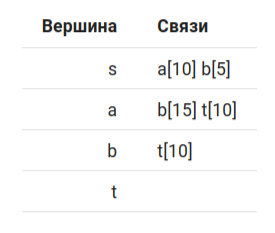
\includegraphics[width=0.6\linewidth]{figs/task-11/adj-ff-2.png}
  \end{minipage}
  \caption{Ориентированный взвешенный граф}
\end{figure}

\begin{minted}{js}
{
  "weighted": true,
  "oriented": true,
  "adj": {
    "source": {
      "a": 10,
      "b": 5
    },
    "a": {
      "b": 15,
      "sink": 10
    },
    "b": {
      "sink": 10
    },
    "t": {}
  }
}
\end{minted}

\subsubsection{Выходные данные}
\begin{figure}[H]
  \centering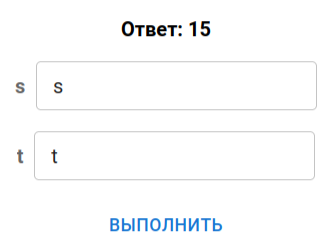
\includegraphics[width=0.3\textwidth]{figs/task-11/res-ff-2.png}
  \caption{Результат работы}
\end{figure}

\subsubsection{Входные данные}
\begin{figure}[H]
  \begin{minipage}{0.5\textwidth}
    \centering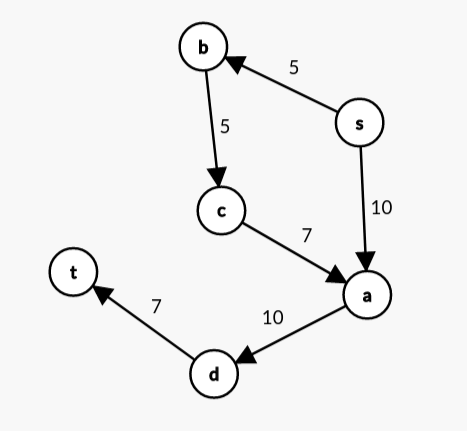
\includegraphics[width=0.8\linewidth]{figs/task-11/graph-ff-3.png}
  \end{minipage}
  \begin{minipage}{0.5\textwidth}
    \centering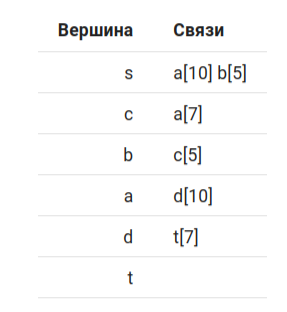
\includegraphics[width=0.6\linewidth]{figs/task-11/adj-ff-3.png}
  \end{minipage}
  \caption{Ориентированный взвешенный граф}
\end{figure}

\begin{minted}{js}
{
  "weighted": true,
  "oriented": true,
  "adj": {
    "s": {
      "a": 10,
      "b": 5
    },
    "c": {
      "a": 7
    },
    "b": {
      "c": 5
    },
    "a": {
      "d": 10
    },
    "d": {
      "t": 7
    },
    "t": {}
  }
}
\end{minted}

\subsubsection{Выходные данные}
\begin{figure}[H]
  \centering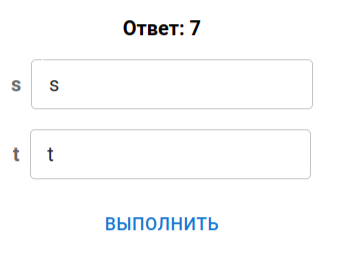
\includegraphics[width=0.3\textwidth]{figs/task-11/res-ff-3.png}
  \caption{Результат работы}
\end{figure}